The implementation of the EMT simulator in VeraGrid involves several steps, including the development of the core simulation engine,
the integration with existing  models, and the creation of user interfaces for configuration and result visualization. Regarding
this project scope, the focus has been placed on the core simulation engine development and device models, and its integration with the existing
dynamic framework. The GUI implementation, then, stays out of scope of this project and awaits as future work to be done.

\subsubsection*{Core simulation development: EMTP combined with the Symbolic-Numeric approach}

The EMT simulation engine is developed in Python, following the general structure of the dynamic simulation framework in VeraGrid. The general simulation structure for any simulation in VeraGrid
 is shown in Figure \ref{fig:General_Simulation_Structure} and widely explained in the subsection \ref{2_2ImplementationSmall}. 

The main class responsible for the EMT simulation is the Driver class, which contains the simulation function itself. 
This function initializes the system, sets up the time-stepping loop, and performs the numerical integration using the EMTP method combined with the Symbolic-Numeric approach.
The core of the simulation consists on solving the MNA equations at each time-step using the EMT method. The aforementioned equation system, also found below is solved.

\begin{equation}
    [\bm{G}]~[\bm{v}(t)] = [\bm{i}(t)]-[\bm{I_{\text{hist}}}]
\end{equation}

The current contributions are computed at each time-step based on the previous steps results and the device models. 
Due to the large variety of models for some devices while some others are standardized, a combined full numeric (traditional EMTP) and
Symbolic-Numeric approach is used in the simulation. This means that some devices such as lines and transformers are modelled using
standardized companion models explained in the previous subsection, while others such as generators are modelled using symbolic equations allowing the user
to define custom models and parameters. This combination provides both flexibility and efficiency in the simulation. However, from a computational perspective,
 Symbolic-Numeric solvers may be slower than fully numerical solvers, particularly when large-scale models are simulated.
  As a result, a trade-off must be considered between providing an easy and user-friendly modelling experience and achieving high computational performance in the solver.

In the context of this thesis, the generator model used is the EMT-type model synchronous machine explained in the previous subsection.

\begin{figure}[h!]
  \centering
  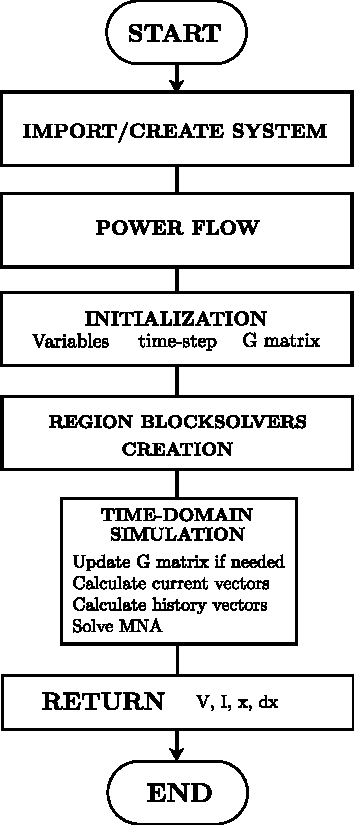
\includegraphics[width=0.35\linewidth]{inkscape_svg/block_diagram_full_EMT_simulation.pdf}
  \caption{EMT simulation block diagram.}
  \label{fig:block_diagram_general_EMT}
\end{figure}

The operations done during an EMT simulation are summarized in Figure~\ref{fig:block_diagram_general_EMT} and widely explained in the following lines.

\begin{itemize}
    \item \textit{Initialization:} The system is initialized following the next steps:
     \begin{itemize}
        \item \textit{Time step adaptation based on the line parameters:} the time-step of the simulation must be a divisor of the largest line delay ($\tau$). The time-step given
        by the user is then adapted to fulfill this requirement. Moreover, if it is too big, a message logger is raised to inform the user.
        \item \textit{Initial guess calculation:} If Symbolic-Numeric models are used, an initial guess of the state variables is needed to start the Newton-Raphson iterations. The bus voltages are obtained from
        the power flow solution, while the rest are obtained from initialization equations defined by each device model. The derivatives of the state variables are all set to 0.0.
        \item \textit{Initial conductance matrix  $G$ assembly:} The conductance matrix $G$ is assembled by adding the contributions of all the devices in the system. The local $G$ matrix for each device is computed when each device is initialized.
        In the case of the branches, a mask system is used to assemble the global $G$ matrix efficiently. It is to be noted that the solver allows any number of phases (including neutral) to each bus. Therefore,
        the size of the $G$ matrix is conditioned to the number of phases of each bus.
     \end{itemize}
    \item \textit{Region Symbolic-Numeric BlockSolvers creation:} To improve the efficiency of the simulation, the system is divided into regions based on the connectivity of Symbolic-Numeric models to each bus. Each bus has its own region composed by all the injections
    with Symbolic-Numeric models connected to it. Then, a BlockSolver is created for each region, which will be used to solve the local equations of the region during the time-stepping loop. In this way, the size of each system block to be solved is reduced and the calculation 
    could be parallelized in future implementations to improve calculation time. A new class called "EMTSolverProperties" is created to store the Blocksolver, parameters, initial guesses and solutions of each region.
    \item \textit{$G$ matrix factorization:} The conductance matrix $G$ is factorized using an LU decomposition to prepare it for the time-stepping loop. 
    \item \textit{Time-stepping loop:} For each time-step, voltages, currents and internal variables from the symbolic-numeric devices are calculated. This is done using the predictor-corrector algorithm: first
    internal variables as well as current sources are calculated using the previous step voltage solution. Using these currents, the MNA is solved and voltages are found. With the new voltages, the variables are corrected again. The following operations are performed to simulate the system dynamics:
        \begin{itemize}
            \item \textit{Predict Isources:} The current sources contributions from the Symbolic-Numeric models are calculated based on the previous step voltage solution. One time-step simulation is performed for each region using the BlockSolver created during initialization. Afterwards,
            the current contributions found in the simulations are assembled into the global current source vector.
            \item \textit{Update history currents:} The line and transformer history currents are updated based on the previous voltage and current solutions. It must be highlighted that in the case of the line,
            the history terms are updated only after the delay time has passed for each line. In the case of the transformers, the history components are updated at each time-step regarding the previous step results.
            \item \textit{Solve MNA equations:} The MNA equation system is solved using the factorized $G$ matrix and the updated current and history contributions. 
            \item \textit{Update (correct) Isources:} The current sources contributions from the Symbolic-Numeric models are calculated based on the recalculated voltage solution. This is done exactly as in 
            \textit{Predict Isources} step but using the updated voltages in order to have the most accurate solution.
            \item \textit{Calculate branch currents:} The currents through each branch are calculated based on the updated voltages. Those are needed in future timesteps.
        \end{itemize}
             Figure \ref{fig:block_diagram_run_EMT} shows the block diagram of the EMT simulation process.
        \begin{figure}[h!]
            \centering
            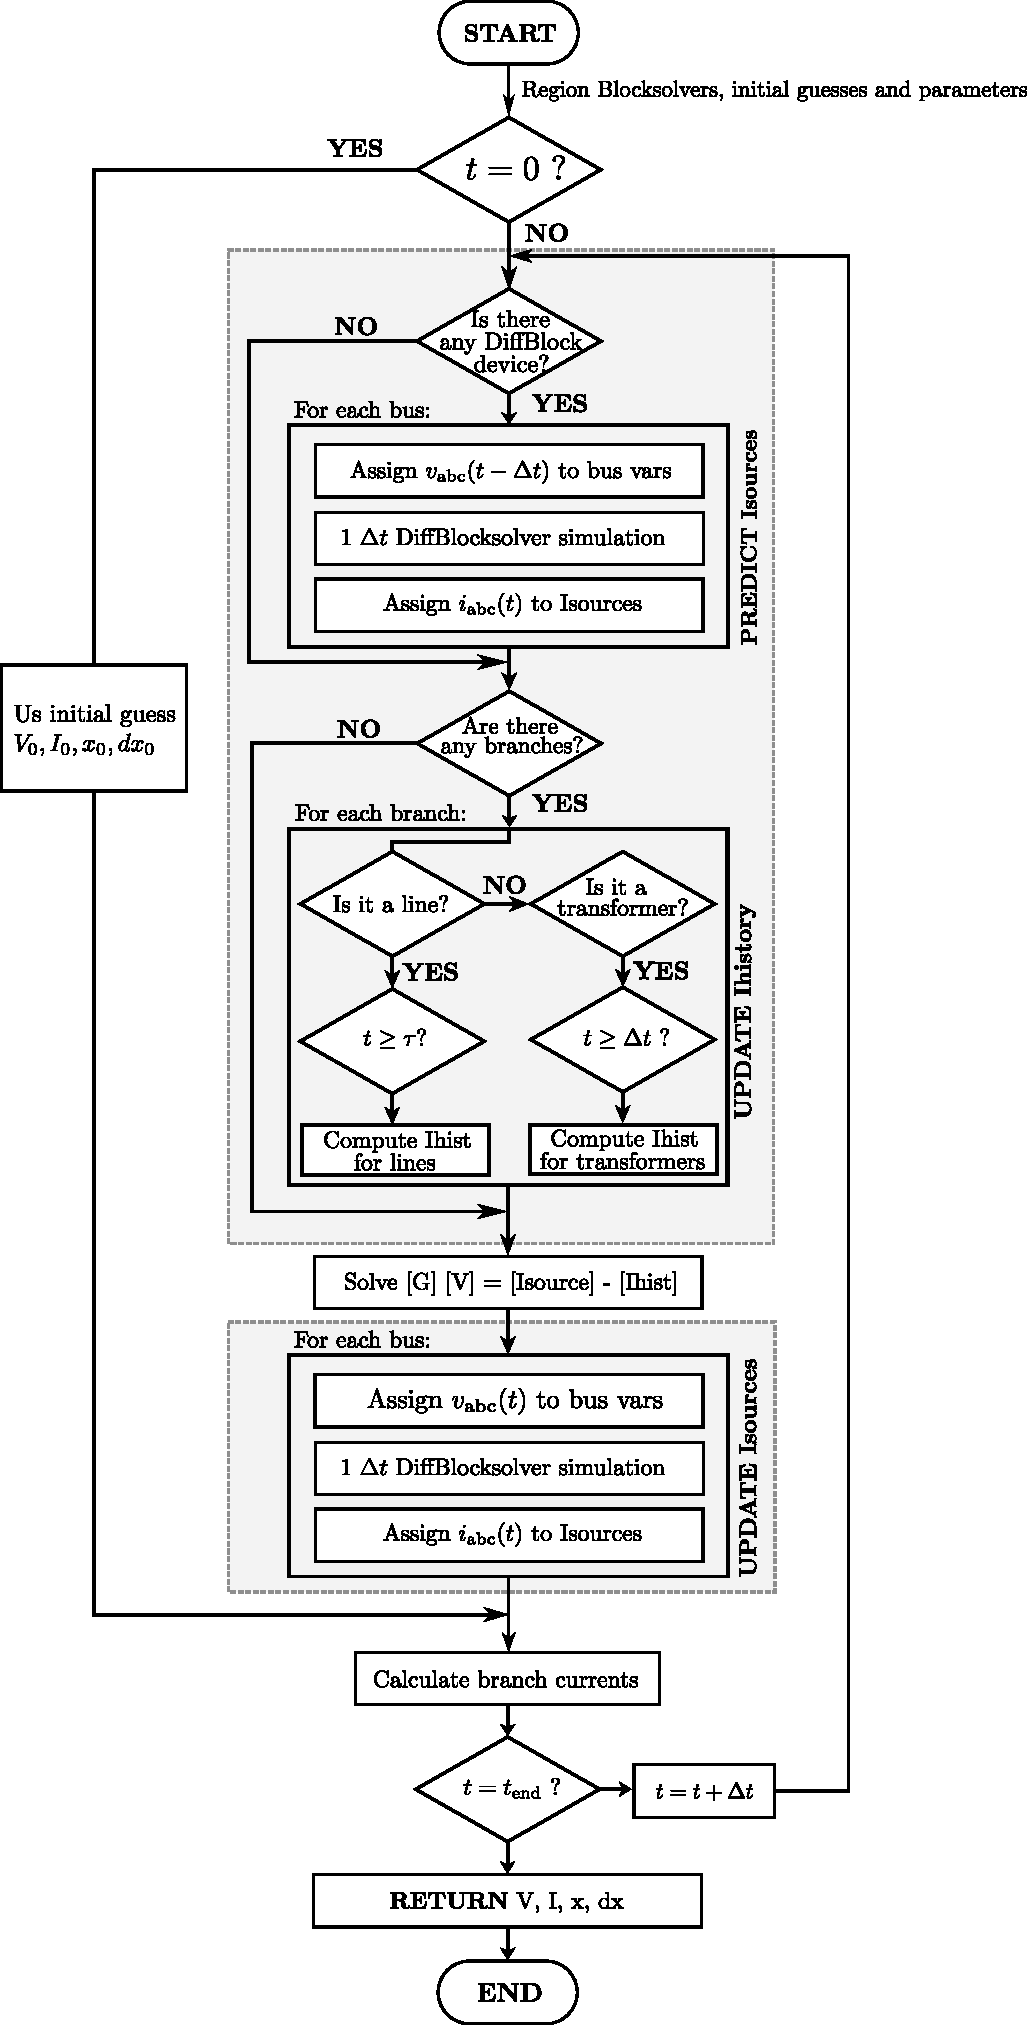
\includegraphics[width=0.66\linewidth]{inkscape_svg/block_diagram_run_EMTP.pdf}
            \caption{EMT simulation block diagram.}
            \label{fig:block_diagram_run_EMT}
        \end{figure}

    \item \textit{Results saving and post-processing:} After the simulation, results are saved in csv files and post-processed for analysis and visualization.
\end{itemize}